\documentclass[tikz,border=8pt]{standalone}
\usetikzlibrary{arrows.meta,fit,positioning}

\begin{document}
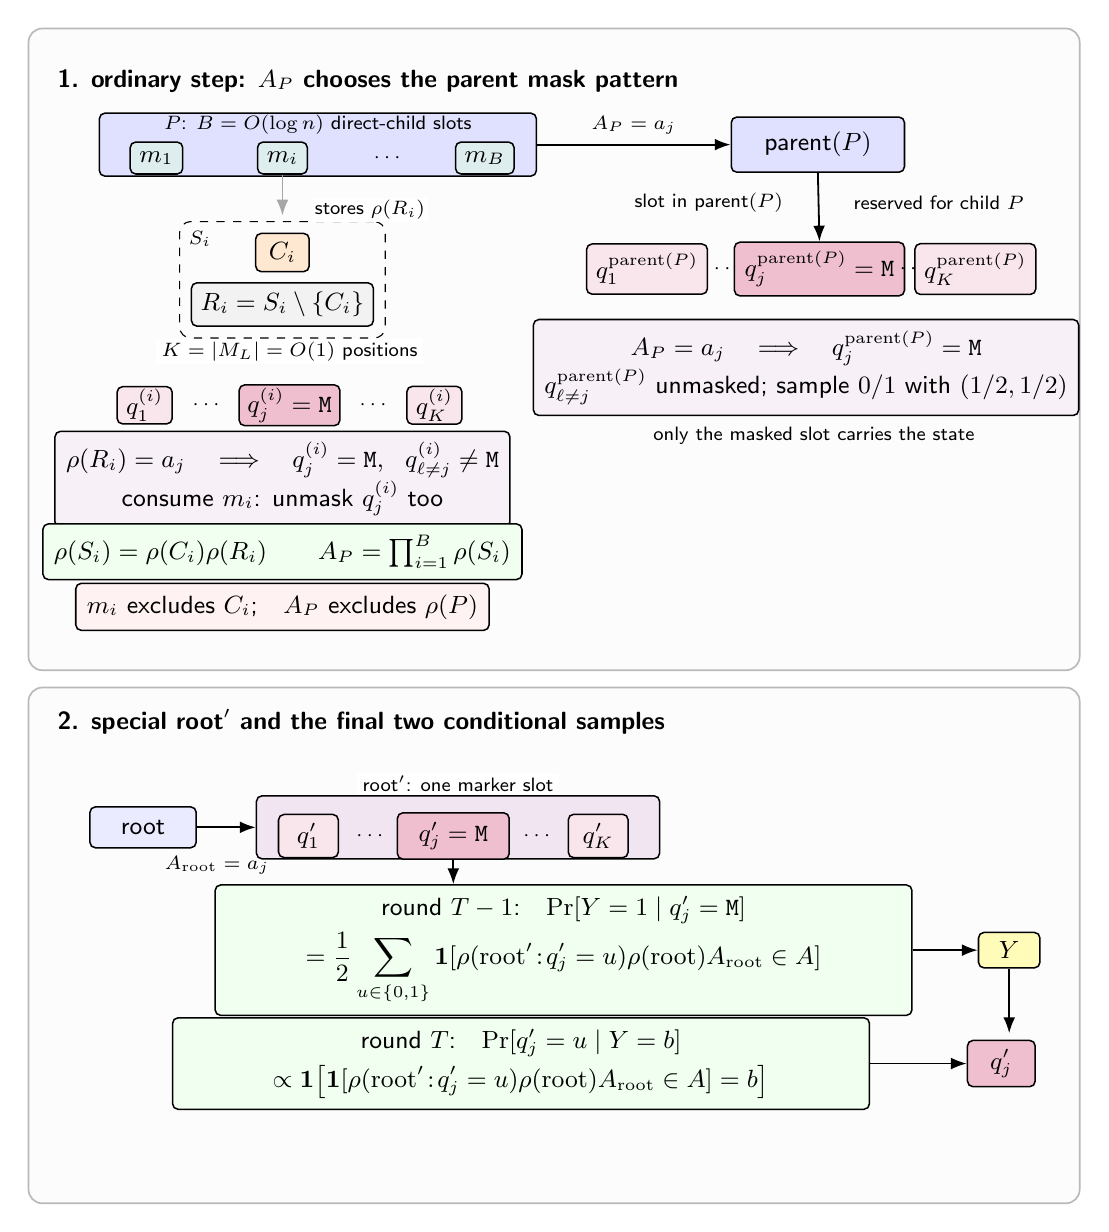
\begin{tikzpicture}[
  font=\sffamily,
  box/.style={draw, rounded corners=2pt, line width=0.55pt, font=\small\sffamily},
  panel/.style={draw=gray!55, rounded corners=5pt, line width=0.6pt, fill=gray!2},
  title/.style={font=\small\sffamily\bfseries},
  small/.style={font=\scriptsize\sffamily},
  tiny/.style={font=\tiny\sffamily},
  nodebox/.style={box, fill=blue!8, minimum height=0.52cm, minimum width=1.35cm},
  parentbox/.style={box, fill=blue!12, minimum height=0.70cm, minimum width=2.20cm},
  coord/.style={box, fill=orange!18, minimum height=0.40cm, minimum width=0.68cm},
  rem/.style={box, fill=gray!10, minimum height=0.40cm, minimum width=1.50cm},
  slot/.style={box, fill=teal!13, minimum height=0.36cm, minimum width=0.58cm},
  qslot/.style={box, fill=purple!10, minimum height=0.38cm, minimum width=0.76cm},
  live/.style={box, fill=purple!25, minimum height=0.40cm, minimum width=1.42cm},
  qmini/.style={qslot, minimum height=0.35cm, minimum width=0.70cm, inner sep=1pt, font=\small\sffamily},
  livemini/.style={live, minimum height=0.37cm, minimum width=1.28cm, inner sep=1pt, font=\small\sffamily},
  ybit/.style={box, fill=yellow!28, minimum height=0.43cm, minimum width=0.78cm},
  formula/.style={box, fill=green!6, inner sep=4pt, align=center, font=\small\sffamily},
  rule/.style={box, fill=violet!6, inner sep=4pt, align=center, font=\small\sffamily},
  note/.style={box, fill=red!5, inner sep=4pt, align=center, font=\small\sffamily},
  captionlabel/.style={font=\scriptsize\sffamily, fill=white, inner xsep=2pt, inner ysep=1pt},
  arrow/.style={-{Latex[length=2mm]}, line width=0.65pt},
  softarrow/.style={-{Latex[length=2mm]}, line width=0.55pt, gray!70}
]

% ---------------------------------------------------------------------------
% Figure 1: ordinary upward step and parent mask pattern.
% ---------------------------------------------------------------------------
\node[panel, minimum width=13.35cm, minimum height=8.15cm] at (0,1.45) {};
\node[title, anchor=west] at (-6.43,4.86)
  {1. ordinary step: $A_P$ chooses the parent mask pattern};

\node[parentbox, minimum width=5.55cm, minimum height=0.80cm] (Pbox) at (-3.00,4.05) {};
\node[small] at (-3.00,4.31) {$P$: $B=O(\log n)$ direct-child slots};
\node[slot] (m1) at (-5.05,3.88) {$m_1$};
\node[slot] (mi) at (-3.45,3.88) {$m_i$};
\node[small] at (-2.12,3.88) {$\cdots$};
\node[slot] (mB) at (-0.88,3.88) {$m_B$};
\node[coord] (Ci) at (-3.45,2.68) {$C_i$};
\node[rem] (Ri) at (-3.45,2.02) {$R_i=S_i\setminus\{C_i\}$};
\node[draw, dashed, rounded corners=4pt, inner sep=4pt, fit=(Ci)(Ri)] (Si) {};
\node[small, anchor=north west] at (Si.north west) {$S_i$};
\draw[softarrow] (mi.south) -- ([yshift=2pt]Si.north);
\node[small, anchor=west, fill=white, inner sep=1pt] at (-3.08,3.22)
  {stores $\rho(R_i)$};

\node[qmini] (qi1) at (-5.20,0.74) {$q^{(i)}_1$};
\node[small] at (-4.42,0.74) {$\cdots$};
\node[livemini] (qij) at (-3.36,0.74) {$q^{(i)}_j=\mathtt M$};
\node[small] at (-2.30,0.74) {$\cdots$};
\node[qmini] (qiK) at (-1.52,0.74) {$q^{(i)}_K$};
\node[captionlabel] at (-3.36,1.42)
  {$K=|M_L|=O(1)$ positions};

\node[rule, minimum width=5.45cm] at (-3.45,-0.20)
  {$\rho(R_i)=a_j
    \quad\Longrightarrow\quad
    q^{(i)}_j=\mathtt M,\ \ q^{(i)}_{\ell\ne j}\ne\mathtt M$\\
   consume $m_i$: unmask $q^{(i)}_j$ too};

\node[formula, minimum width=5.25cm] at (-3.45,-1.12)
  {$\rho(S_i)=\rho(C_i)\rho(R_i)$\qquad
   $A_P=\prod_{i=1}^{B}\rho(S_i)$};
\node[note, minimum width=5.25cm] at (-3.45,-1.82)
  {$m_i$ excludes $C_i$;\quad $A_P$ excludes $\rho(P)$};

\node[parentbox, minimum width=2.20cm] (Parent) at (3.35,4.05) {parent$(P)$};
\draw[arrow] (Pbox.east) -- node[small, above] {$A_P=a_j$} (Parent.west);

\node[small, anchor=east] at (3.03,3.31)
  {slot in parent$(P)$};
\node[small, anchor=west] at (3.68,3.31)
  {reserved for child $P$};
\node[qslot, minimum width=1.06cm] (qp1) at (1.18,2.47)
  {$q^{\mathrm{parent}(P)}_1$};
\node[small] at (2.20,2.47) {$\cdots$};
\node[live, minimum width=2.16cm] (qpj) at (3.37,2.47)
  {$q^{\mathrm{parent}(P)}_j=\mathtt M$};
\node[small] at (4.56,2.47) {$\cdots$};
\node[qslot, minimum width=1.06cm] (qpK) at (5.35,2.47)
  {$q^{\mathrm{parent}(P)}_K$};
\draw[arrow] (Parent.south) -- (qpj.north);

\node[rule, minimum width=6.35cm] at (3.20,1.22)
  {$A_P=a_j\quad\Longrightarrow\quad
    q^{\mathrm{parent}(P)}_j=\mathtt M$\\
   $q^{\mathrm{parent}(P)}_{\ell\ne j}$ unmasked; sample $0/1$ with $(1/2,1/2)$};
\node[small, align=center] at (3.30,0.36)
  {only the masked slot carries the state};

% ---------------------------------------------------------------------------
% Figure 2: special top aggregation and final two conditional samples.
% ---------------------------------------------------------------------------
\node[panel, minimum width=13.35cm, minimum height=6.55cm] at (0,-6.12) {};
\node[title, anchor=west] at (-6.43,-3.28)
  {2. special root$'$ and the final two conditional samples};

\node[nodebox] (root) at (-5.22,-4.62) {root};
\node[parentbox, fill=violet!10, minimum width=5.12cm, minimum height=0.80cm] (rootpBlock) at (-1.22,-4.62) {};
\node[captionlabel, anchor=south] at (rootpBlock.north)
  {root$'$: one marker slot};
\node[qslot] (r1) at (-3.12,-4.73) {$q'_1$};
\node[small] at (-2.34,-4.73) {$\cdots$};
\node[live] (rj) at (-1.28,-4.73) {$q'_j=\mathtt M$};
\node[small] at (-0.22,-4.73) {$\cdots$};
\node[qslot] (rK) at (0.56,-4.73) {$q'_K$};
\draw[arrow] (root.east) -- (rootpBlock.west);
\node[small] at (-4.28,-5.10) {$A_{\mathrm{root}}=a_j$};

\node[formula, minimum width=8.85cm] (fy) at (0.12,-6.18)
  {round $T-1$:\quad
    $\Pr[Y=1\mid q'_j=\mathtt M]$\\[2pt]
    $\displaystyle
    ={1\over2}\sum_{u\in\{0,1\}}
    \mathbf{1}[
      \rho(\mathrm{root}'\!:\!q'_j=u)\rho(\mathrm{root})A_{\mathrm{root}}\in A]$};
\node[ybit] (Y) at (5.78,-6.18) {$Y$};
\draw[arrow] (rj.south) -- (rj |- fy.north);
\draw[arrow] (fy.east) -- (Y.west);

\node[formula, minimum width=8.85cm] (fq) at (-0.42,-7.62)
  {round $T$:\quad
    $\Pr[q'_j=u\mid Y=b]$\\[2pt]
    $\displaystyle
    \propto
    \mathbf{1}\!\left[
      \mathbf{1}[
        \rho(\mathrm{root}'\!:\!q'_j=u)\rho(\mathrm{root})A_{\mathrm{root}}\in A]=b
    \right]$};
\node[live, minimum width=0.86cm] (Qsample) at (5.68,-7.62) {$q'_j$};
\draw[arrow] (Y.south) -- ++(0,-0.82);
\draw[arrow] (fq.east) -- (Qsample.west);

\end{tikzpicture}
\end{document}
